% ----------------------------------------------------------
% GESTÃO DE TEMPO / CRONOGRAMA
% ----------------------------------------------------------
\section{Cronograma}

No início do projeto tínhamos uma organização dos macro itens (\textit{Epics}) que precisavam ser desenvolvidos com base nas entregas da disciplina de PI1A5 e dentro dos \textit{Epics} estipulamos as tarefas a serem feitas. Por meio do \gls{jira} podemos ter uma visão geral do andamento dos \textit{Epics} e os prazos, além das \textit{\glspl{sprint}} planejadas, realizadas e aquela que está em andamento.

\begin{figure}[H]
	\centering
	\caption{\label{jira-geral}Roteiro Geral de PI1A5}
	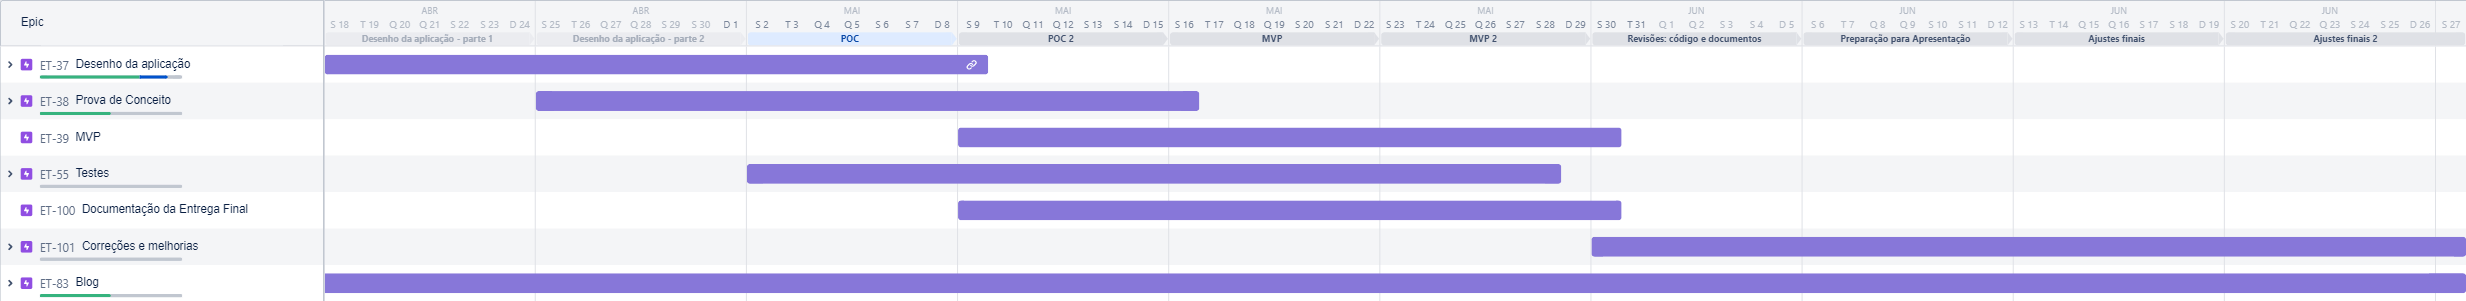
\includegraphics[width=0.95\textwidth]{../imagens/cronograma-geral.png}
	\fonte{Os Autores}
\end{figure}

A \autoref{jira-geral} mostra à esquerda a lista dos \textit{Epics} considerados para a construção do sistema \emph{EstagiEI} no início do projeto, começando pelo Desenho da Aplicação, então Prova de Conceito, \ac{mvp}, Testes, Documentação da Entrega Final, Correções e Melhorias e Blog. Na parte superior estão as datas e o período englobado por cada \textit{\gls{sprint}}. As marcações em azul mostram o período de duração de cada \textit{Epic}. A seguir, \autoref{jira-detalhe1} e \autoref{jira-detalhe2} mostram de modo mais próximo a figura anterior para fins de melhor visualização.

\begin{figure}[H]
	\centering
	\caption{\label{jira-detalhe1}Roteiro Geral de PI1A5 - Detalhe Inicial}
	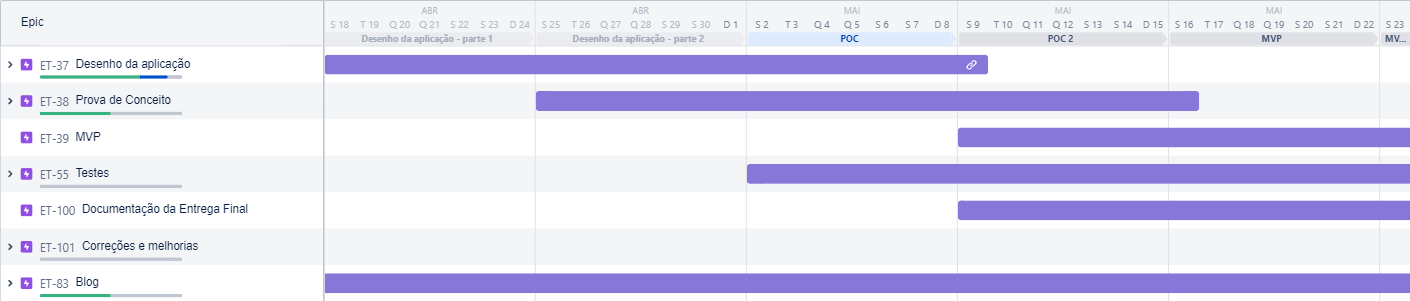
\includegraphics[width=0.95\textwidth]{../imagens/cronograma-detalhe1.png}
	\fonte{Os Autores}
\end{figure}

\begin{figure}[H]
	\centering
	\caption{\label{jira-detalhe2}Roteiro Geral de PI1A5 - Detalhe Final}
	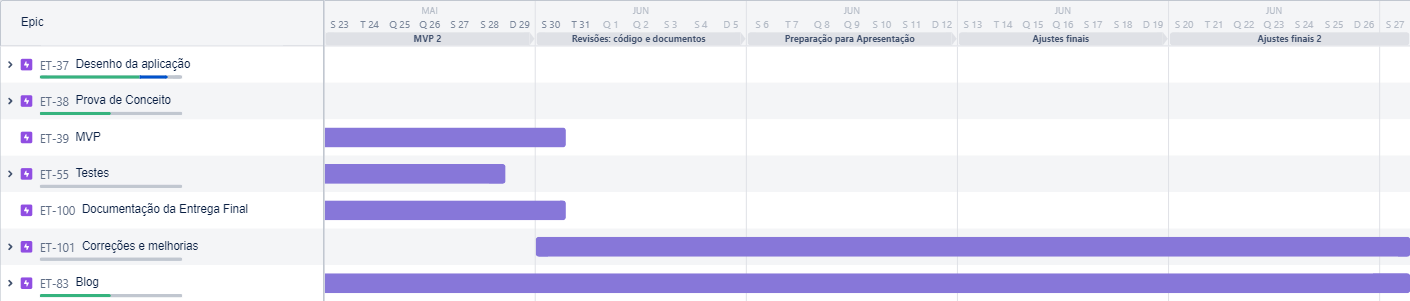
\includegraphics[width=0.95\textwidth]{../imagens/cronograma-detalhe2.png}
	\fonte{Os Autores}
\end{figure}

Apresentamos em \autoref{cronogramasem1} as \textit{\glspl{sprint}} e algumas informações expostas em \autoref{jira-geral}, \autoref{jira-detalhe1} e \autoref{jira-detalhe2} do que foi planejado e realizado em PI1A5.

\begin{quadro}[H]
	\caption{Cronograma de \glspl{sprint} - 1º semestre}
	\centering
	\begin{tabular}{| p{0.17\linewidth}  | c | c | p{0.25\linewidth} | c |}
		\hline
		\thead[l]{Sprint} & \thead{Data Inicial} & \thead{Data Final} & \thead[l]{Descrição} & \thead{Status}\\
		\hline
		Desenho da aplicação 1 & 18/04/22 & 25/04/22 & Elaboração da documentação do Desenho da Aplicação. & Concluída\\
		\hline
		Desenho da aplicação 2 & 25/04/22 & 02/05/22 &  Continuação da elaboração do Desenho da Aplicação. Planejamento para a \ac{poc}. & Concluída\\
		\hline
		POC & 02/05/22 & 09/05/22 & Finalização do Desenho da Aplicação. Início do desenvolvimento dos itens da \ac{poc} & Concluída \\
		\hline
		POC 2 & 09/05/22 & 16/05/22 & Continuação do desenvolvimento dos itens da \ac{poc}. & Concluída\\
		\hline
		MVP & 16/05/22 & 23/05/22 & Aproveitamento do que foi desenvolvido para a \ac{poc} com melhorias e ampliação conforme possível para o \ac{mvp}. & Concluída\\
		\hline
		MVP 2 & 23/05/22 & 30/05/22 & Continuação do trabalho no desenvolvimento do \ac{mvp}. & Concluída\\
		\hline
		Revisões: código e documentos & 30/05/22 & 06/06/22 &  Finalização e revisão tanto do desenvolvimento quanto da documentação. & Concluída\\
		\hline
		Preparação para a Apresentação & 06/06/22 & 13/06/22 &  Organização e planejamento da apresentação do projeto e sua documentação. & Concluída\\
		\hline
		Ajustes finais & 13/06/22 & 20/06/22 &  Ajustes a serem feitos para correção e/ou melhoria do projeto apresentado. & Concluída\\
		\hline
		Ajustes finais 2 & 20/06/22 & 27/06/22 &  Continuação de correções e ajustes para a entrega do projeto no semestre. & Concluída\\
		\hline
		Ajustes finais 3 & 27/06/22 & 04/07/22 &  Finalização dos ajustes finais e correções para a entrega definitiva do projeto no semestre. & Concluída\\
		\hline
		
	\end{tabular}
	\fonte{Os Autores}
	\label{cronogramasem1}
\end{quadro}

Para a continuação do projeto, percebemos que uma mudança de planejamento seria necessária. Assim, modificamos nossos \textit{Epics} a fim de estarem mais alinhados com o projeto em desenvolvimento, possuindo subitens de Funcionalidades que se referem a partes menores do produto em si, as quais por sua vez contém as Histórias de Usuário, que descrevem as ações/funções de cada usuário dentro so sistema.

Como o \gls{jira} não possui uma divisão intermediária entre \textit{Epics} e Histórias de Usuário, a seguir apresentamos alguns esquemas da visão que temos das divisões do projeto:

\begin{figure}[H]
	\centering
	\caption{\label{epic-empresa}\textit{Epic} da Empresa}
	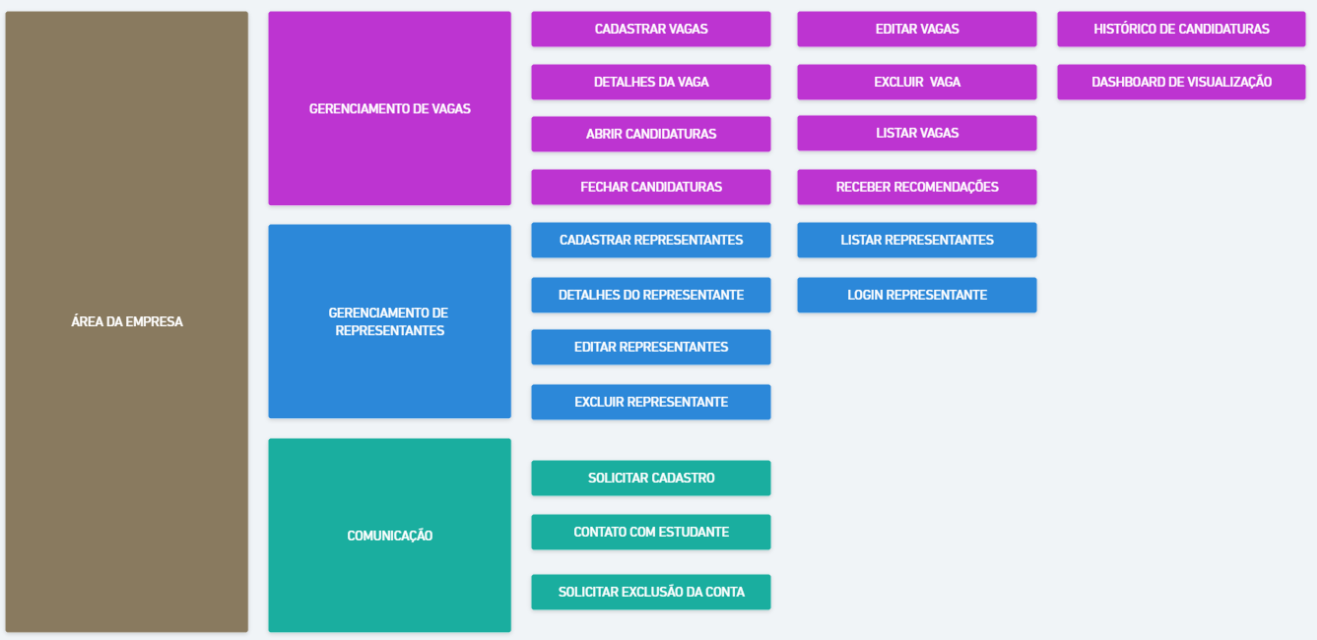
\includegraphics[width=0.95\textwidth]{../imagens/epic-empresa.png}
	\fonte{Os Autores}
\end{figure}

Em \autoref{epic-empresa} está a Área da Empresa, que seria uma grande fatia do projeto, contendo as Funcionalidades pertinentes a entidade Empresa e o que se relaciona com ela, como o Gerenciamento de Vagas, o qual se abre em diversas ações que são as Histórias de Usuário dessa funcionalidade.

\begin{figure}[H]
	\centering
	\caption{\label{epic-estudante}\textit{Epic} do Estudante}
	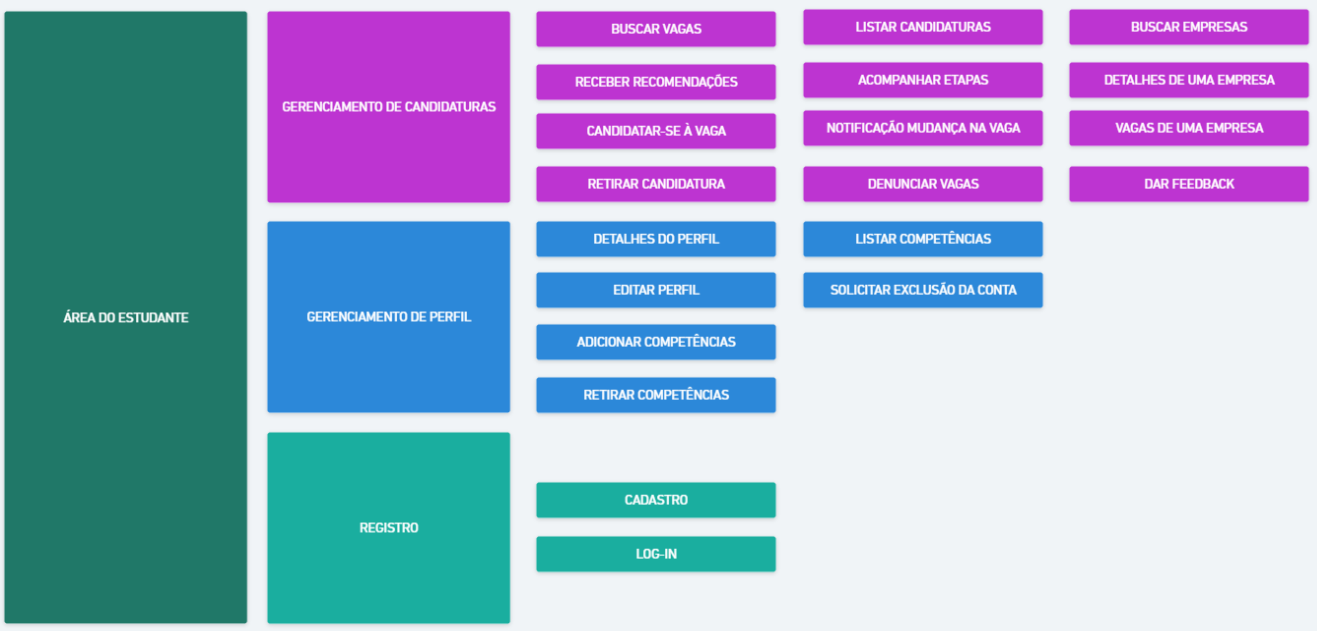
\includegraphics[width=0.95\textwidth]{../imagens/epic-estudante.png}
	\fonte{Os Autores}
\end{figure}

Do mesmo modo como o \textit{Epic} da Empresa, o \textit{Epic} do Estudante também possui Funcionalidades pertinentes a entidade Estudante e as ações que um usuário deste tipo precisa ter no sistema, como o Gerenciamento de Candidaturas.

Além de reestruturarmos o modo como vemos e trabalhamos as etapas do projeto, também adaptamos as \textit{\glspl{sprint}} para serem de duas semanas ao invés de uma, devido à situação de tempo dos membros da equipe. O \autoref{jira-roteiro-geral-sem2} ilustra a nova organização de \textit{Epics} dividas entre \gls{backend} e \gls{frontend} e as \textit{\glspl{sprint}} de suas semanas.

\begin{figure}[H]
	\centering
	\caption{\label{jira-roteiro-geral-sem2}Roteiro Geral para PI2A6}
	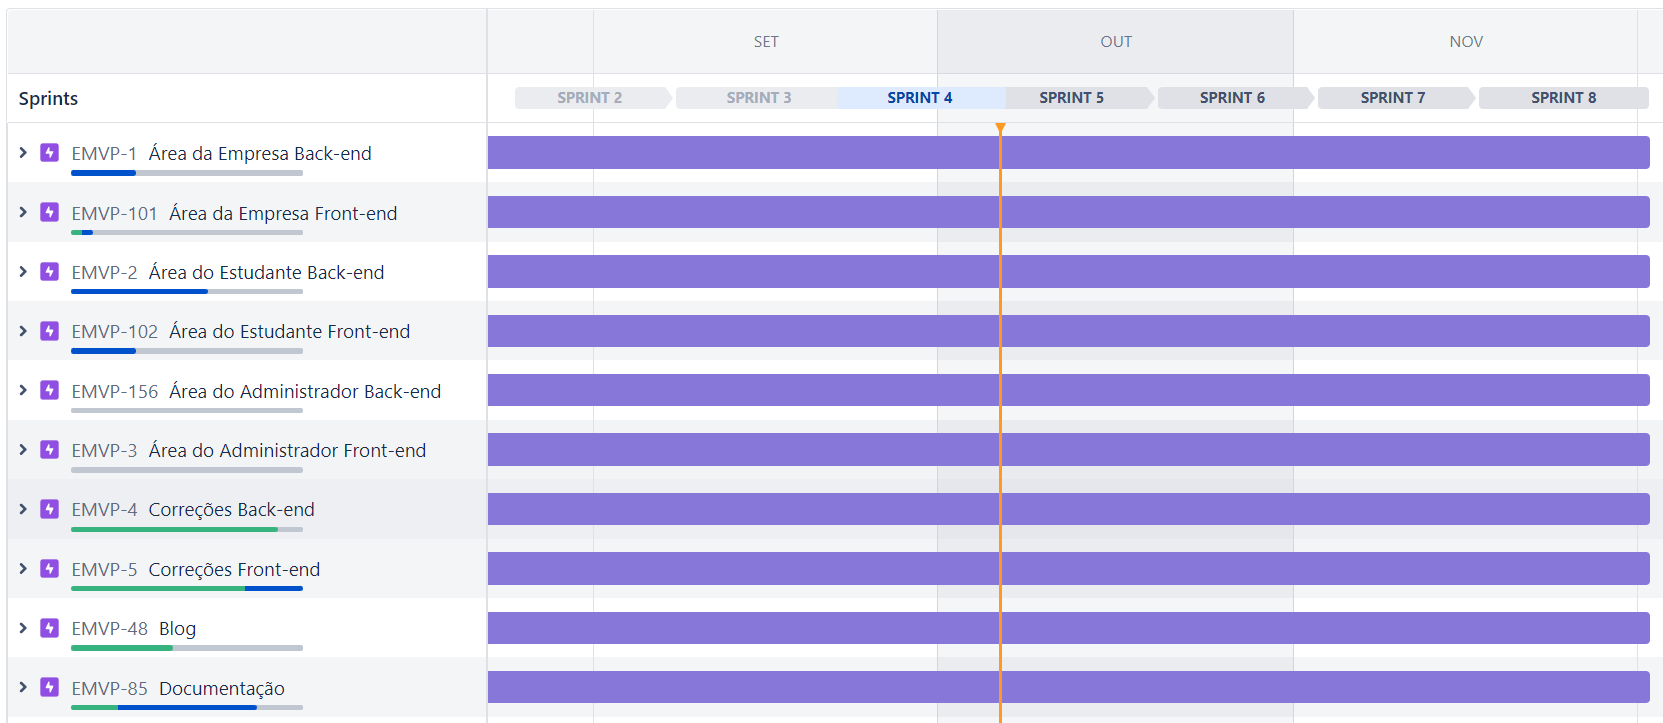
\includegraphics[width=0.95\textwidth]{../imagens/jira-roteiro-geral-sem2.png}
	\fonte{Os Autores}
\end{figure}

Considerando tudo o que já foi apontado, nosso Cronograma (a seguir) se tornou mais genérico, pois a cada \gls{sprint} definimos o que seria feito, portanto apenas há algo definido explicitamente no início e no fim da segunda etapa de desenvolvimento, como a entrega final.

\begin{quadro}[H]
	\caption{Cronograma de \glspl{sprint} - 2º semestre}
	\centering
	\begin{tabular}{| p{1.5cm}  | c | c | p{4.5cm} | c |}
		\hline
		\thead[l]{Sprint} & \thead{Data Inicial} & \thead{Data Final} & \thead[l]{Descrição} & \thead{Status}\\
		\hline
		\textit{Sprint} 1 & 11/08/22 & 25/08/22 & Reorganização da equipe, reestruturação do código e do projeto de modo geral & Concluída\\
		\hline
		\textit{Sprint} 2 & 25/08/22 & 08/09/22 &  Refinamento, ajustes e adaptações do que já foi produzido; adequação da documentação existente às alterações & Concluída\\
		\hline
		\textit{Sprint} 3 & 08/09/22 & 22/09/22 & Desenvolvimento e testes de novas funcionalidades do sistema & Concluída \\
		\hline
		\textit{Sprint} 4 & 22/09/22 & 06/10/22 & Desenvolvimento e testes de novas funcionalidades do sistema & Concluída\\
		\hline
		\textit{Sprint} 5 & 06/10/22 & 20/10/22 & Desenvolvimento e testes de novas funcionalidades do sistema & Concluída\\
		\hline
		\textit{Sprint} 6 & 20/10/22 & 03/11/22 & Desenvolvimento e testes de novas funcionalidades do sistema & Concluída\\
		\hline
		\textit{Sprint} 7 & 03/11/22 & 17/11/22 & Ajustes finais, Entrega e Apresentação da aplicação & Em Progresso\\
		\hline
		\textit{Sprint} 8 & 17/11/22 & 01/12/22 & Correções e ajustes; Entrega final & Não Iniciada\\
		\hline
		
	\end{tabular}
	\fonte{Os Autores}
	\label{cronogramasem2}
\end{quadro}